% !TeX root = ../../Book3.tex
% 纲要标题：### 24.4 临界集中与紧性
% 纲要位置：几何学计划纲要.md，第 3149 行。
% 正文状态：初稿；尚未正式审核。

% 纲要内容开始
% 
% * Euclid 气泡与尺度不变性
% * 范数分裂与能量缺陷
% * 低于球面常数时排除集中
% * 严格阈值下的极小值实现
% 
% 纲要内容结束

\section{临界集中与紧性}
\label{g3:sec:2404}

非正情形中，能量的符号帮助保住了极小化序列的质量。正情形需要更精确的信息：一个缩小到点附近的函数，至少要付出多少梯度能量？答案由 Euclid 空间的最佳 Sobolev 常数决定；共形对应又把这个常数识别为圆球的 Yamabe 常数。本节用范数分裂与能量比较证明严格阈值下的紧性。

\subsection{Euclid 气泡与尺度不变性}
\label{g3:subsec:2404:01}
固定 \(n\ge3\)，仍记 \(p=2n/(n-2)\)、\(a_n=4(n-1)/(n-2)\)。在 \(\mathbb R^n\) 上考虑
\begin{equation}\label{g3:eq:yamabe-euclidean-bubble}
	U_\varepsilon(x)=\left(\frac{\varepsilon}{\varepsilon^2+|x|^2}\right)^{(n-2)/2}
	=\varepsilon^{-(n-2)/2}U_1(x/\varepsilon),\qquad\varepsilon>0.
\end{equation}
这类函数称为\term[linjie qipao]{临界气泡}[critical bubble]。参数变小时，峰值增加、有效宽度缩小。换元 \(x=\varepsilon y\) 给出
\[
	\int_{\mathbb R^n}U_\varepsilon^p\,\mathrm dx
	=\int_{\mathbb R^n}U_1^p\,\mathrm dx,
	\qquad
	\int_{\mathbb R^n}|\mathrm DU_\varepsilon|^2\,\mathrm dx
	=\int_{\mathbb R^n}|\mathrm DU_1|^2\,\mathrm dx.
\]
两个积分都是有限正数。这里不要求 \(U_\varepsilon\in L^2(\mathbb R^n)\)：在 \(n=3,4\) 时，该条件恰好失败。临界变分首先控制的是梯度的 \(L^2\) 范数与函数的 \(L^p\) 范数。

\begin{figure}[htbp]
	\centering
	% !TeX root = ../Book3.tex
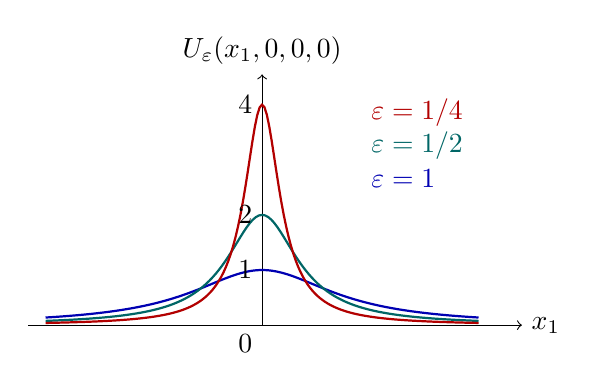
\begin{tikzpicture}[x=1.1cm,y=0.7cm]
	\draw[->] (-2.7,0)--(3.0,0) node[right] {\(x_1\)};
	\draw[->] (0,0)--(0,4.55) node[above] {\(U_\varepsilon(x_1,0,0,0)\)};
	\draw[thick,blue!70!black,domain=-2.5:2.5,samples=141] plot (\x,{1/(1+\x*\x)});
	\draw[thick,teal!80!black,domain=-2.5:2.5,samples=141] plot (\x,{0.5/(0.25+\x*\x)});
	\draw[thick,red!70!black,domain=-2.5:2.5,samples=181] plot (\x,{0.25/(0.0625+\x*\x)});
	\node[left] at (0,1) {\(1\)};
	\node[left] at (0,2) {\(2\)};
	\node[left] at (0,4) {\(4\)};
	\node[blue!70!black,right] at (1.15,2.65) {\(\varepsilon=1\)};
	\node[teal!80!black,right] at (1.15,3.25) {\(\varepsilon=1/2\)};
	\node[red!70!black,right] at (1.15,3.85) {\(\varepsilon=1/4\)};
	\node[below left] at (0,0) {\(0\)};
\end{tikzpicture}

	\caption[临界气泡的尺度变化]{四维时 \(U_\varepsilon(x)=\varepsilon/(\varepsilon^2+|x|^2)\) 的一条径向截面。三条曲线的峰高和宽度不同；保持不变的是四维积分 \(\int_{\mathbb R^4}U_\varepsilon^4\)，而非图中曲线下的平面面积。}
	\label{g3:fig:yamabe-bubbles}
\end{figure}

确定梯度能量的最小代价，需要如下锐形式。它是本节使用的外部分析结果；见\cite[定理3.3，第50页]{LeeParker1987Yamabe}。
\begin{theorem}[锐 Sobolev 不等式]\label{g3:thm:yamabe-sharp-euclidean}
	设 \(n\ge3\)，令
	\[
		Y_S\coloneqq n(n-1)\operatorname{Vol}(S^n,g_{\mathrm{rd}})^{2/n},
	\]
	其中 \(g_{\mathrm{rd}}\) 是截面曲率为一的圆球度量。对每个 \(v\in C_c^\infty(\mathbb R^n)\)，有
	\begin{equation}\label{g3:eq:yamabe-sharp-sobolev}
		Y_S\left(\int_{\mathbb R^n}|v|^p\,\mathrm dx\right)^{2/p}
		\le a_n\int_{\mathbb R^n}|\mathrm Dv|^2\,\mathrm dx.
	\end{equation}
	常数 \(Y_S\) 不能增大。不等式延伸到 \(C_c^\infty\) 关于梯度 \(L^2\) 范数的完备化，在该空间中，式\eqref{g3:eq:yamabe-euclidean-bubble}的函数取得等号。
\end{theorem}
锐常数及气泡等号由所引文献第3节提供。本节从这一精确版本出发，证明它对紧流形极小化序列的后果。完备化中的函数可由式\eqref{g3:eq:yamabe-sharp-sobolev}唯一地解释为 \(L^p\) 函数，因此上述延伸有明确的函数意义。

\begin{proposition}\label{g3:prop:yamabe-sphere-constant}
	对 \(n\ge3\) 的单位圆球，有 \(Y(S^n,[g_{\mathrm{rd}}])=Y_S\)。
\end{proposition}
\begin{proof}
	立体投影把去掉一点的圆球度量写成
	\[
		g_{\mathrm{rd}}=\rho^{4/(n-2)}g_{\mathrm{eucl}},\qquad
		\rho(x)=\left(\frac{2}{1+|x|^2}\right)^{(n-2)/2}.
	\]
	给定光滑 \(w\) 于圆球，记它在这个坐标中的表达仍为 \(w\)，并令 \(F=\rho w\)。\Cref{g3:prop:conformal-laplacian-covariance}的共形能量变换给出
	\[
		\int_{\mathbb R^n}|F|^p\,\mathrm dx
		=\int_{S^n}|w|^p\,\mathrm d\mu_{\mathrm{rd}},
		\qquad
		a_n\int_{\mathbb R^n}|\mathrm DF|^2\,\mathrm dx=E_{g_{\mathrm{rd}}}(w).
	\]
	为核对无穷远处的积分，圆球上的光滑性给出 \(F=O(r^{2-n})\)、\(\mathrm DF=O(r^{1-n})\)。取在 \(B_R\) 上为一、支于 \(B_{2R}\)、梯度不超过 \(C/R\) 的截断 \(\eta_R\)。则 \(\eta_RF\to F\) 于 \(L^p\)，且梯度差的平方积分为 \(O(R^{2-n})\)。因此可以先对紧支函数使用共形公式与分部积分，再令 \(R\to\infty\)；没有留下边界项。

	对 \(\eta_RF\) 应用锐 Sobolev 不等式并取极限，得到 \(Q_{g_{\mathrm{rd}}}(w)\ge Y_S\)。光滑稠密性把它推广到 \(H^1(S^n)\)。另一方面，\(s_{g_{\mathrm{rd}}}=n(n-1)\)，常函数一满足
	\[
		Q_{g_{\mathrm{rd}}}(1)
		=n(n-1)\operatorname{Vol}(S^n,g_{\mathrm{rd}})^{1-2/p}=Y_S.
	\]
	上下界一致。
\end{proof}

现在把气泡放进任意闭流形的一个小坐标球。这个构造同时给出上界与失紧序列，因而解释了为什么必须关注严格不等号。
\begin{proposition}\label{g3:prop:yamabe-bubble-upper-bound}
	设 \((M^n,g)\) 为闭连通光滑黎曼流形，\(n\ge3\)。则 \(Y(M,[g])\le Y_S\)。此外，存在非负 \(v_\varepsilon\in C^\infty(M)\)，满足
	\[
		\|v_\varepsilon\|_p=1,\qquad
		v_\varepsilon\rightharpoonup0\ \text{于 }H^1(M),\qquad
		Q_g(v_\varepsilon)\longrightarrow Y_S.
	\]
	这些函数没有 \(L^p\) 强收敛子列。
\end{proposition}
\begin{proof}
	取一点 \(x_0\) 的正规坐标球 \(B_{2r}(0)\)，以及在 \(B_r\) 上为一、支于 \(B_{2r}\) 的光滑非负截断 \(\chi\)。把 \(b_\varepsilon=\chi U_\varepsilon\) 搬到 \(M\)，在坐标球外补零。换元后，\(g_{ij}(\varepsilon y)\to\delta_{ij}\) 于每个固定球，且原坐标球上的度量与 Euclid 度量一致可比。利用 \(U_1^p\) 和 \(|\mathrm DU_1|^2\) 的可积性，先控制 \(|y|>R\) 的尾部，再令 \(\varepsilon\to0\)、\(R\to\infty\)，得到
	\[
		\int_M b_\varepsilon^p\,\mathrm d\mu_g\longrightarrow
		A\coloneqq\int_{\mathbb R^n}U_1^p\,\mathrm dx>0,
	\qquad
		\int_M|\mathrm db_\varepsilon|^2\,\mathrm d\mu_g
		\longrightarrow\int_{\mathbb R^n}|\mathrm DU_1|^2\,\mathrm dx.
	\]
	第二个极限中的截断误差支于固定环带，在那里 \(U_\varepsilon\) 及其导数均为 \(O(\varepsilon^{(n-2)/2})\)，故误差趋于零。

	零阶项要单独估计。径向积分给出
	\begin{equation}\label{g3:eq:yamabe-bubble-l2}
		\|b_\varepsilon\|_2^2\le C
		\begin{cases}
			\varepsilon,&n=3,\\
			\varepsilon^2\log(1/\varepsilon),&n=4,\\
			\varepsilon^2,&n\ge5,
		\end{cases}
	\end{equation}
	其中取 \(0<\varepsilon<\min\{r,1/2\}\)。例如换元后的积分是常数倍的
	\(\varepsilon^2\int_0^{2r/\varepsilon}t^{n-1}(1+t^2)^{-(n-2)}\,\mathrm dt\)；被积函数在无穷远处为 \(O(t^{3-n})\)，所以出现以上三种情形。由于 \(s_g\) 有界，\(\int s_gb_\varepsilon^2\to0\)。锐不等式在 \(U_1\) 上取等号，遂有 \(Q_g(b_\varepsilon)\to Y_S\)。

	取 \(v_\varepsilon=b_\varepsilon/\|b_\varepsilon\|_p\)。它们在 \(H^1\) 中有界而在 \(L^2\) 中趋于零，因此每个弱收敛子列的极限都为零，故整族弱趋于零。若存在 \(L^p\) 强收敛子列，它也在 \(L^2\) 中趋于同一极限零，与 \(L^p\) 范数恒为一矛盾。最后，由 \(Y(M,[g])\le Q_g(v_\varepsilon)\) 取极限即得上界。
\end{proof}

在任意远离 \(x_0\) 的紧集上，\(v_\varepsilon\) 及其梯度都趋于零；与此同时，\(\int v_\varepsilon^p=1\)。也就是说，体积密度 \(v_\varepsilon^p\,\mathrm d\mu_g\) 的质量集中到 \(x_0\)。这具体说明了临界约束为什么不由弱收敛保留。

\subsection{范数分裂与能量缺陷}
\label{g3:subsec:2404:02}
为处理一般极小化序列，并不需要预先证明它只含一个气泡。只要把弱极限与余项分开，给余项一个带锐常数的能量下界，就足以排除质量丢失。首先把 Euclid 不等式局部化；低阶误差留在 \(L^2\) 项中，而这个范数已有 Rellich 紧性。

\begin{lemma}\label{g3:lem:yamabe-near-sharp-sobolev}
	设 \((M^n,g)\) 为闭光滑黎曼流形，\(n\ge3\)。对每个 \(0<\delta<Y_S\)，存在 \(C_\delta\)，使每个 \(v\in H^1(M)\) 满足
	\begin{equation}\label{g3:eq:yamabe-near-sharp-sobolev}
		(Y_S-\delta)\|v\|_p^2
		\le a_n\|\mathrm dv\|_2^2+C_\delta\|v\|_2^2.
	\end{equation}
\end{lemma}
\begin{proof}
	以充分小的正规坐标球覆盖 \(M\)。度量系数及体积密度与 Euclid 值一致接近，故锐 Euclid 不等式与范数比较说明，对每个支于其中一球的 \(f\)，都有
	\[
		(Y_S-\delta)\|f\|_{L^p(g)}^2\le a_n\|\mathrm df\|_{L^2(g)}^2.
	\]
	这里选球的大小时，将两个比较因子的乘积控制得足够接近一，即可达到给定 \(\delta\)。取从属于有限覆盖的光滑函数 \(\eta_i\)，使 \(\sum_i\eta_i^2=1\)。它们可以从普通单位分解 \(\psi_i\) 构造为 \(\eta_i=\psi_i/(\sum_j\psi_j^2)^{1/2}\)。

	因为 \(p/2>1\)，\(L^{p/2}\) 的三角不等式给出
	\[
		\|v\|_p^2
		=\left\|\sum_i(\eta_iv)^2\right\|_{p/2}
		\le\sum_i\|\eta_iv\|_p^2.
	\]
	局部估计求和后，使用 \(\sum_i\eta_i\,\mathrm d\eta_i=0\)，得到精确恒等式
	\[
		\sum_i|\mathrm d(\eta_iv)|^2
		=|\mathrm dv|^2+v^2\sum_i|\mathrm d\eta_i|^2.
	\]
	最后一项的系数在紧流形上有界，吸收到 \(C_\delta\) 即得结论。先对光滑函数计算，再用 \(H^1\) 光滑稠密性与连续嵌入推广到全部 \(H^1\) 函数。
\end{proof}

下一条范数分裂说明，几乎处处收敛比单纯弱收敛多保留了什么：临界质量虽可能丢失，却可以准确归入余项。
\begin{lemma}\label{g3:lem:yamabe-norm-splitting}
	设 \((X,\mu)\) 为测度空间，\(1<q<\infty\)。若实函数列 \(f_j\) 在 \(L^q(X)\) 中有界，且几乎处处趋于 \(f\)，则 \(f\in L^q(X)\)，并有
	\begin{equation}\label{g3:eq:yamabe-norm-splitting}
		\int_X|f_j|^q\,\mathrm d\mu
		=\int_X|f|^q\,\mathrm d\mu
		+\int_X|f_j-f|^q\,\mathrm d\mu+o(1).
	\end{equation}
\end{lemma}
\begin{proof}
	Fatou 引理给出 \(f\in L^q\)，故 \(h_j=f_j-f\) 也在 \(L^q\) 中有界。对每个 \(\epsilon>0\)，中值公式和 Young 不等式给出
	\[
		\bigl||a+b|^q-|a|^q\bigr|
		\le\epsilon|a|^q+C_\epsilon|b|^q,
		\qquad a,b\in\mathbb R.
	\]
	具体地，中值公式先给出 \(C_q(|a|^{q-1}|b|+|b|^q)\)，再用共轭指数 \(q/(q-1)\) 与 \(q\) 即得所示形式。令
	\[
		d_j=|f_j|^q-|h_j|^q-|f|^q,
		\qquad r_j=(|d_j|-\epsilon|h_j|^q)_+.
	\]
	由于 \(h_j\to0\) 几乎处处，有 \(r_j\to0\) 几乎处处；上式又给 \(0\le r_j\le(C_\epsilon+1)|f|^q\)。支配收敛定理于是给出 \(\int r_j\to0\)。因此
	\[
		\limsup_j\int_X|d_j|\,\mathrm d\mu
		\le\epsilon\sup_j\|h_j\|_q^q.
	\]
	令 \(\epsilon\downarrow0\) 即得 \(d_j\to0\) 于 \(L^1\)，从而得到所需等式。
\end{proof}

\begin{lemma}\label{g3:lem:yamabe-energy-defect}
	设 \((M^n,g)\) 为闭光滑黎曼流形，\(n\ge3\)。设实函数 \(u_j\rightharpoonup u\) 于 \(H^1(M)\)，\(\|u_j\|_p=1\)，且 \(E_g(u_j)\to\ell\)。则
	\begin{equation}\label{g3:eq:yamabe-energy-defect}
		\ell\ge E_g(u)+Y_S(1-\|u\|_p^p)^{2/p}.
	\end{equation}
\end{lemma}
\begin{proof}
	由\cref{g3:thm:compact-bundle-rellich}，弱收敛列在 \(L^2\) 中强趋于 \(u\)；取子列后也几乎处处收敛。写 \(w_j=u_j-u\)。前一引理给出
	\[
		\|w_j\|_p^p\longrightarrow1-\|u\|_p^p\ge0.
	\]
	弱收敛使梯度交叉项趋于零，\(L^2\) 强收敛使所有含 \(s_g\) 的余项趋于零。因此
	\[
		E_g(u_j)=E_g(u)+a_n\|\mathrm dw_j\|_2^2+o(1).
	\]
	对 \(w_j\) 使用式\eqref{g3:eq:yamabe-near-sharp-sobolev}，先令 \(j\to\infty\)；因为 \(\|w_j\|_2\to0\)，得到
	\[
		\ell-E_g(u)\ge(Y_S-\delta)(1-\|u\|_p^p)^{2/p}.
	\]
	再令 \(\delta\downarrow0\)，得到结论。各个子列产生同一个不等式，所以取几乎处处收敛子列不影响断言。
\end{proof}

这就是本章所需的\term[jizhong jin xing]{集中紧性}[concentration compactness]估计：余项携带的临界质量为 \(1-\|u\|_p^p\)，它的能量至少为这份质量的 \(2/p\) 次幂乘以 \(Y_S\)。证明没有预设余项的空间形状，因而也涵盖多个区域中的集中。

\subsection{低于球面常数时排除集中}
\label{g3:subsec:2404:03}
记 \(Y=Y(M,[g])\)，并令 \(\alpha=2/p=(n-2)/n\in(0,1)\)。若 \(\|u_j\|_p=1\)、\(E_g(u_j)\to Y\)，能量缺陷估计与 \(E_g(u)\ge Y\|u\|_p^2\) 将给出
\begin{equation}\label{g3:eq:yamabe-mass-comparison}
	Y\ge Yt^\alpha+Y_S(1-t)^\alpha,
	\qquad t=\|u\|_p^p\in[0,1].
\end{equation}
这里 \(t=0\) 表示所有临界质量都离开弱极限，\(0<t<1\) 表示只保住一部分，\(t=1\) 表示没有丢失。下面的代数比较同时处理这三种可能。

\begin{lemma}\label{g3:lem:yamabe-threshold-exclusion}
	设 \(Y<Y_S\)、\(Y_S>0\)、\(0<\alpha<1\)。若 \(t\in[0,1]\) 满足式\eqref{g3:eq:yamabe-mass-comparison}，则 \(t=1\)。
\end{lemma}
\begin{proof}
	若 \(t=0\)，式子给出 \(Y\ge Y_S\)，矛盾。若 \(0<t<1\) 且 \(Y>0\)，则
	\[
		Yt^\alpha+Y_S(1-t)^\alpha
		>Y\bigl(t^\alpha+(1-t)^\alpha\bigr)>Y,
	\]
	因为 \(t^\alpha>t\)、\((1-t)^\alpha>1-t\)。若 \(Y\le0\)，则
	\[
		Yt^\alpha+Y_S(1-t)^\alpha-Y
		=Y(t^\alpha-1)+Y_S(1-t)^\alpha>0;
	\]
	第一项非负，第二项为正。这同样与假设矛盾。只剩 \(t=1\)。
\end{proof}

严格阈值有两个作用。全部集中时，代价 \(Y_S\) 已经高于极小值 \(Y\)；部分集中时，指数 \(\alpha<1\) 又使质量拆分增加代价。这解释了为何不必先定位集中点，也能证明极小化序列紧。

\subsection{严格阈值下的极小值实现}
\label{g3:subsec:2404:04}
\begin{theorem}\label{g3:thm:yamabe-below-sphere}
	设 \((M^n,g)\) 为闭连通光滑黎曼流形，\(n\ge3\)，且
	\[
		Y(M,[g])<Y(S^n,[g_{\mathrm{rd}}])=Y_S.
	\]
	则存在光滑正函数 \(u\)，使 \(\int_Mu^p\,\mathrm d\mu_g=1\)、\(E_g(u)=Y(M,[g])\)。它满足
	\[
		L_gu=Y(M,[g])u^{p-1},
	\]
	度量 \(u^{4/(n-2)}g\) 具有体积一和常标量曲率 \(Y(M,[g])\)。每个归一化的非负极小化序列，都有在 \(H^1(M)\) 中强收敛到某个这样的极小函数的子列。
\end{theorem}
\begin{proof}
	记 \(Y=Y(M,[g])\)，取非负极小化序列 \(u_j\)，满足 \(\|u_j\|_p=1\)。Hölder 不等式给出 \(\|u_j\|_2^2\le\operatorname{Vol}(M,g)^{2/n}\)，而
	\[
		a_n\|\mathrm du_j\|_2^2
		\le E_g(u_j)+\|s_g^-\|_\infty\|u_j\|_2^2,
		\qquad s_g^-=\max\{-s_g,0\}.
	\]
	故 \(u_j\) 在 \(H^1\) 中有界。取弱收敛子列 \(u_j\rightharpoonup u\)，由 Rellich 紧性进一步取 \(L^2\) 及几乎处处收敛子列。因此 \(u\ge0\)，且 \(t=\|u\|_p^p\le1\)。

	由能量缺陷估计以及 Yamabe 常数的定义，得到式\eqref{g3:eq:yamabe-mass-comparison}；当 \(u=0\) 时，\(E_g(u)\ge Y\|u\|_p^2\) 也成立。\Cref{g3:lem:yamabe-threshold-exclusion}给出 \(t=1\)。于是 \(u\) 保留全部约束，且
	\[
		Y\le E_g(u)\le\liminf_jE_g(u_j)=Y.
	\]
	这里第二个不等式使用梯度范数弱下半连续性与势能项的 \(L^2\) 连续性。所以 \(u\) 取得极小值。

	还有强收敛。由 \(E_g(u_j)\to E_g(u)\) 及 \(L^2\) 强收敛，得到 \(\|\mathrm du_j\|_2\to\|\mathrm du\|_2\)。Hilbert 空间中的弱收敛与范数收敛推出梯度强收敛，结合 \(L^2\) 收敛即得 \(H^1\) 强收敛。连续 Sobolev 嵌入同时给出 \(L^p\) 强收敛。

	\Cref{g3:prop:yamabe-euler-lagrange}的约束变分给出所示弱方程，\(u\not\equiv0\)。\Cref{g3:thm:yamabe-weak-regularity}把它提升为光滑正解；共形标量曲率及体积公式给出度量的结论。对任意归一化非负极小化序列，上述步骤都适用，故也得到最后的紧性断言。
\end{proof}

\begin{example}\label{g3:exm:yamabe-threshold-sharpness}
	在圆球上，\(Y=Y_S\)，极小值已由常函数取得；但\cref{g3:prop:yamabe-bubble-upper-bound}给出的截断气泡仍是归一化极小化序列，并且弱趋于零。因此，极小值存在不意味着所有极小化序列紧。严格阈值定理同时证明存在性与序列紧性，而等号情形至少需要另行处理其中的集中行为。
\end{example}

至此，剩余问题集中为一个几何比较：除圆球共形类之外，如何把某个测试函数的商压到 \(Y_S\) 以下？普通坐标中的截断气泡只给极限上界；严格改进要使用曲率展开或 Green 函数的整体信息。
% 纲要条目排为编号小节标题，并进入目录与书签；说明段仍保留于纲要注释中。
